\documentclass{beamer}
\mode<presentation>
\usetheme{CambridgeUS}
\usepackage[russian]{babel}
\usepackage[utf8]{inputenc}
\usepackage[T2A]{fontenc}
\usepackage{sansmathaccent}

\usepackage{verbatim}
\usepackage{alltt}

\pdfmapfile{+sansmathaccent.map}
\title[Итерционные методы]{Итерационные методы}
\author{Наумов Д.А., доц. каф. КТ}
\date[31.10.2019] {Программирование и алгоритмические языки, 2019}

\begin{document}

%ТИТУЛЬНЫЙ СЛАЙД
\begin{frame}
  \titlepage
\end{frame}
  
%СОДЕРЖАНИЕ ЛЕКЦИИ
\begin{frame}
  \frametitle{Содержание лекции}
  \tableofcontents  
\end{frame}

\section{Итерационные методы}

\subsection{Вычисление суммы бесконечного ряда}

\begin{frame}{Итерационные методы}
\begin{block}{Итерационные методы}
методы приближенного решения задач прикладной математики, основанные на последовательном приближении к решению путем многократного применения какой-либо вычислительной процедуры.
\end{block}
В данной теме итерационные алгоритмы используются при:
\begin{itemize}
\item вычислении функций с использованием рядов;
\item уточнении корней уравнений;
\item численном интегрировании.
\end{itemize}
\end{frame} 

\begin{frame}{Итерационные методы}
Общая схема итерационного процесса:
\begin{figure}[h]
\centering
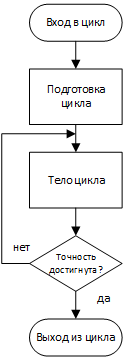
\includegraphics[scale=0.75]{images/lec05-pic01.png}
\end{figure}
\end{frame} 

\begin{frame}{Итерационные методы}
Из-за различных ошибок
\begin{itemize}
\item ошибок ввода исходных данных;
\item ошибок программирования;
\item ошибок времени выполнения; 
\end{itemize}
могут возникать зацикливания – \textbf{бесконечно повторяемые вычисления}
\end{frame}

\begin{frame}
Схема итерационного процесса с ограничением количества итераций:
\begin{figure}[h]
\centering
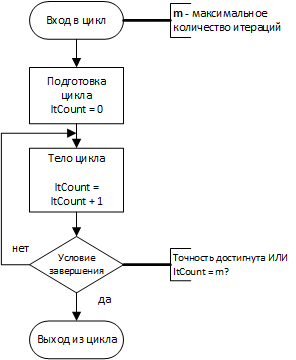
\includegraphics[scale=0.75]{images/lec05-pic02.png}
\end{figure}
\end{frame} 

\begin{frame}{Итерационные методы}
\begin{itemize}
\item Максимальное число итераций \textit{m} должно гарантировать достижение заданной точности вычислений. 
\item Фактическое число повторений цикла определяется величиной допустимой погрешности, а не значением \textit{m}. 
\item Если в теле цикла или в проверяемом условии будут ошибки, приводящие к зацикливанию, то повторения будут
прекращены при достижении счетчиком итераций ItCount предельного значения.
\end{itemize}
\end{frame}

\begin{frame}{Вычисление суммы ряда}
При вычислении значения функции с использованием функционального ряда:
\[\sum\limits_{n=1}^\infty f_n(x)=f_1(x)+f_2(x)+...+f_n(x)\]
задача сводится к последовательному вычислению частичных сумм $S_1(x), S_2(x),..., S_n(x)$, где 
\[S_n(x)=\sum\limits_{i=1}^n f_i(x)\]
Для сходящегося ряда существует предел 
\[\lim\limits_{n\to \infty} S_n(x)=S(x)\]
где $S(x)$ - сумма функционального ряда.
\end{frame}

\begin{frame}
При вычислении суммы ряда с точностью до слагаемого, не превышающего $\varepsilon$, в качестве окончательного результата принимается значение частичной суммы $S_n(x)$, для которой выполняется условие:
\[|f_n(x)<\varepsilon|\]
Процесс вычисления суммы определяется рекуррентным соотношением:
\[S_n(x)=S_{n-1}(x)+f_n(x)\]
\begin{itemize}
\item суммирование считается законченным при выполнении условия достижения заданной точности. 
\item начальное значение суммы принимается равным нулю.
\end{itemize}
В общем случае начальное значение номера члена ряда может быть отличным от единицы (например, равным нулю). Обозначив его через k, получим:
\[S(x)=\sum\limits_{n=k}^\infty f_n(x)\]
\end{frame}

\begin{frame}
Алгоритм вычисления суммы функционального ряда:
\begin{figure}[h]
\centering
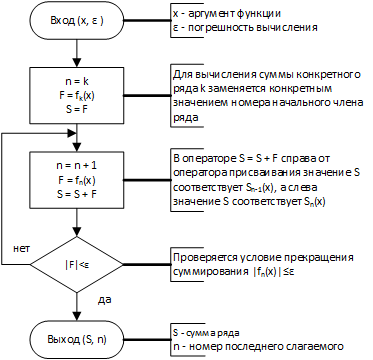
\includegraphics[scale=0.75]{images/lec05-pic03.png}
\end{figure}
\end{frame} 

\begin{frame}
Обычно формула общего члена ряда $f_n(x)$ принадлежит к одному из следующих видов:
\begin{enumerate}
\item $\frac{cos{nx}}{n}$, $\frac{sin(2n-1)x}{2n-1}$;
\item $\frac{x^n}{n!}$, $(-1)^n\frac{x^{2n+1}}{(2n+1)!}$;
\item $\frac{x^{4n+1}}{4n+1}$, $(-1)^n\frac{cos{nx}}{n^2}$;
\end{enumerate}
\begin{block}{Ряд вида 1}
\[f_n(x)=\frac{sin(2n-1)x}{2n-1}\]
формула общего члена содержит только функции, которые можно непосредственно вычислить, т. е. функции, определенные в языке программирования. Вычисления будут наиболее эффективными, если каждый член ряда вычислять по его общей формуле. \end{block}
Вычисление ряда в этом случае организуется по схеме алгоритма с предыдущего слайда.
\end{frame}

\begin{frame}
\begin{block}{Ряд вида 2}
\[f_n(x)=(-1)^n\frac{x^{2n+1}}{(2n+1)!}\]
в формулу общего члена ряда входят только целые степени и факториалы.
\end{block}
Для вычисления $f_n(x)$ используется рекуррентное соотношение: очередной член ряда $f_n(x)$ вычисляется через предыдущий $f_{n-1}(x)$ по формуле 
\[f_n(x) = f_{n-1}(x)\cdot \varphi_n(x)\]
где $\varphi_n(x)$ – переходный коэффициент – функция от $n$ и $х$.
\end{frame}

\begin{frame}
Рассчитаем функцию - переходный коэффициент для следующего ряда:
\[S(x)= \sum\limits_{n=0}^\infty \frac{x^{2n+1}}{(2n+1)!}\]

Вычисления:
\[f_n(x)=\frac{x^{2n+1}}{(2n+1)!}\]
\[f_{n-1}(x)=\frac{x^{2(n-1)+1}}{(2(n-1)+1)!}=\frac{x^{2n-1}}{(2n-1)!}\]
\[\varphi_n(x)=\frac{f_n(x)}{f_{n-1}(x)}= \frac{x^{2n+1}(2n-1)!}{(2n+1)!x^{2n-1}}=\frac{x^2}{2n(2n+1)}\]
\end{frame}

\begin{frame}
Алгоритм вычисления суммы функционального ряда:
\begin{figure}[h]
\centering
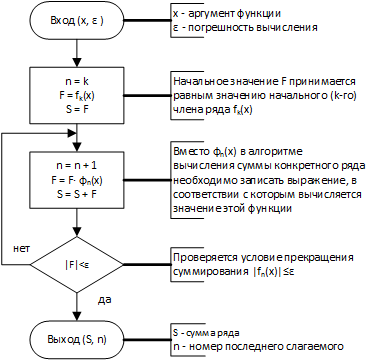
\includegraphics[scale=0.75]{images/lec05-pic04.png}
\end{figure}
\end{frame}

\begin{frame}
\begin{block}{Ряд вида 3}
\[f_n(x)=\frac{x^{n}}{n!}cos(n\frac{\pi}{4})\]
в формулу общего члена ряда входят как функции, вычисляемые непосредственно, так и функции, которые можно вычислить только по рекуррентной формуле. 
\end{block}
Для вычисления $f_n(x)$ бщий член ряда целесообразно представить в виде двух сомножителей: 
\[f_n(x)=c_n(x)\cdot t_n(x)\]
где $c_n(x)$ содержит только элементарные функции и вычисляется непосредственно, а $t_n(x)$ содержит целые степени и факториалы и вычисляется рекуррентно через предыдущее значение.
\end{frame}

\begin{frame}
Рассчитаем функции $c_n(x)$ и $t_n(x)$ для следующего ряда:
\[S(x)= \sum\limits_{n=0}^\infty \frac{x^{n}}{n!}cos(n\frac{\pi}{4})\]

Вычисления:
\[f_n(x)=c_n(x)\cdot t_n(x)\]
\[с_n(x)=cos(n\frac{\pi}{4})\]
\[t_n(x)=\frac{x^n}{n!}\]
Для рекуррентной части $t_n(x)$ вычисляем переходной коэффициент: 
\[\varphi_n(x)=\frac{f_n(x)}{f_{n-1}(x)}= \frac{x^{n}(n-1)!}{n!x^{n-1}}=\frac{x}{n}\]
\end{frame}

\begin{frame}
Алгоритм вычисления суммы функционального ряда:
\begin{figure}[h]
\centering
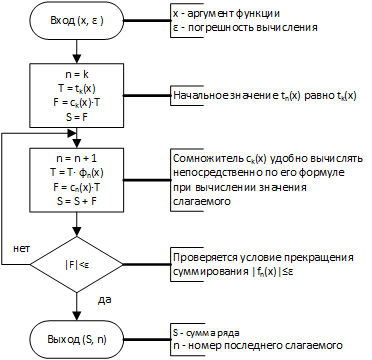
\includegraphics[scale=0.75]{images/lec05-pic05.png}
\end{figure}
\end{frame}

%\subection{Метод итераций для уточнения корней}
%\subsection{Численное интегрирование}

\end{document}
